\documentclass[spanish]{article}
\usepackage[T1]{fontenc}
\usepackage[latin9]{inputenc}
\usepackage[letterpaper]{geometry}
\geometry{verbose,tmargin=2cm,bmargin=2cm,lmargin=2cm,rmargin=2cm,headheight=1cm,headsep=1cm,footskip=1cm}
\usepackage{float}
\usepackage{graphicx}
\usepackage{esint}
\usepackage{babel}
\begin{document}
\title{EV\_1\_5\_caracteristicas de los convertidores de potencia CA-CD, CD-CA, CA-CA
y CD-CD.}

\author{Joel Alejandro Alcantar Diaz.}
\date{16 de septiebre de 2019}
\maketitle
\begin{center}

\includegraphics[scale=0.5]{1.png}\linebreak{}
\par\end{center}

Universidad Politecnica de la Zona Metropolitana de Guadalajara |
Ingenieria Mecatr\'onica | 4to ``A''\pagebreak{}
\begin{center}
\textbf{\LARGE{}Concepto de un convertidor.}{\LARGE\par}
\par\end{center}

Un convertidor de energ\'ia es un sistema o equipo electr\'onico que tiene
por objetivo la convercion de energ\'ia el\'ectrica entre dos formatos
diferentes. Por ejemplo obtener corriente continua a partir de corriente
alterna.\\

\begin{center}
\textbf{\LARGE{}Convertidor CA-CD}{\LARGE\par}
\par\end{center}

Convertidor AC-CD tambien llamado rectificador, es un tipo de convertidor
que tranforma la corriente alterna ya sea trif\'asica o monof\'asica en
corriente directa.\\

Caracteristicas:
\begin{itemize}
\item Alimetan circuitos de exitacion e inducidos.
\item Puede rectificar media onda y onda completa.
\item El control es escalar y vectorial.
\item Funcionan como paso previo a los tranformadores CD-CA de frecuencia
y tencion fija.
\item Se requiere para el control de motores paso a paso.
\end{itemize}
La formula de voltaje de salida promedio es:

\[
Vcd=\frac{2}{T}\int_{0}^{\frac{2}{T}}Vmsen*\omega t
\]

\begin{figure}[H]
\begin{centering}
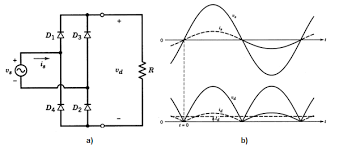
\includegraphics[scale=0.5]{2.png}
\par\end{centering}
\begin{centering}
\caption{Funcionamiento de un rectificador de onda completa.}
\par\end{centering}
\end{figure}

\begin{center}
\textbf{\LARGE{}Convertidor CD-CA.}{\LARGE\par}
\par\end{center}

Los convertidores CD-CA son tambien llamados inversores y su funcion
principal es transformar la corriente directa en alterna.\\

Caracteristicas:
\begin{itemize}
\item Se puede controlar la frecuencia y la tension.
\item Reciben una onda cuadrada y la hacen senoidal
\item Tienen comutacion inperfecta.
\item Pueden perder mucha potencia.
\end{itemize}
\begin{center}
\textbf{\LARGE{}Convertidor CD-CD}{\LARGE\par}
\par\end{center}

Este se se puede considerar como una fuente elevadora o reductura
de voltaje.\\

\begin{itemize}
\item Reductores:
\end{itemize}
En este convertidor el voltaje de entrada siempre sera mayor al de
salida.
\begin{itemize}
\item Elevador
\end{itemize}
En el elevador de voltaje la entrada de tensi\'on siempre sera menor
a la salida.
\begin{itemize}
\item C\'uk
\end{itemize}
Este regulado, nombrado asi por su inventor, entrega un voltaje que
puede ser menor o mayor al de la entrada pero su polaridad es opuesta
al de entrada.
\begin{itemize}
\item Reductore-Elevadores
\end{itemize}
Este tipo de regulador puede elevar o disminuir el voltaje, al igual
que el C\'uk su salida es inversa a la entrada.\\

\begin{center}
\textbf{\LARGE{}Convertidor CA-CA}{\LARGE\par}
\par\end{center}

Caracteristicas:
\begin{itemize}
\item Realizan conversi\'on AC-AC de forma directa y sin etapa intermedia
de continua.
\item Los tristores no necesitan bloqueo forzado gracias al paso natural
por cero de la intensidad.
\item Proporcionan una tencion de frecuencia fundamental menor o igual que
la frecuencia de la tensi\'on de entrada.
\item Proporcionan una tencion con un cierto numero de armonicos.
\end{itemize}
\pagebreak{}
\begin{thebibliography}{siam}

\bibitem{Bibliografia}

\end{thebibliography}


\end{document}
